\subsection{Room temperature measurement}

\subsubsection{Resistivity}
\begin{figure}
    \centering
    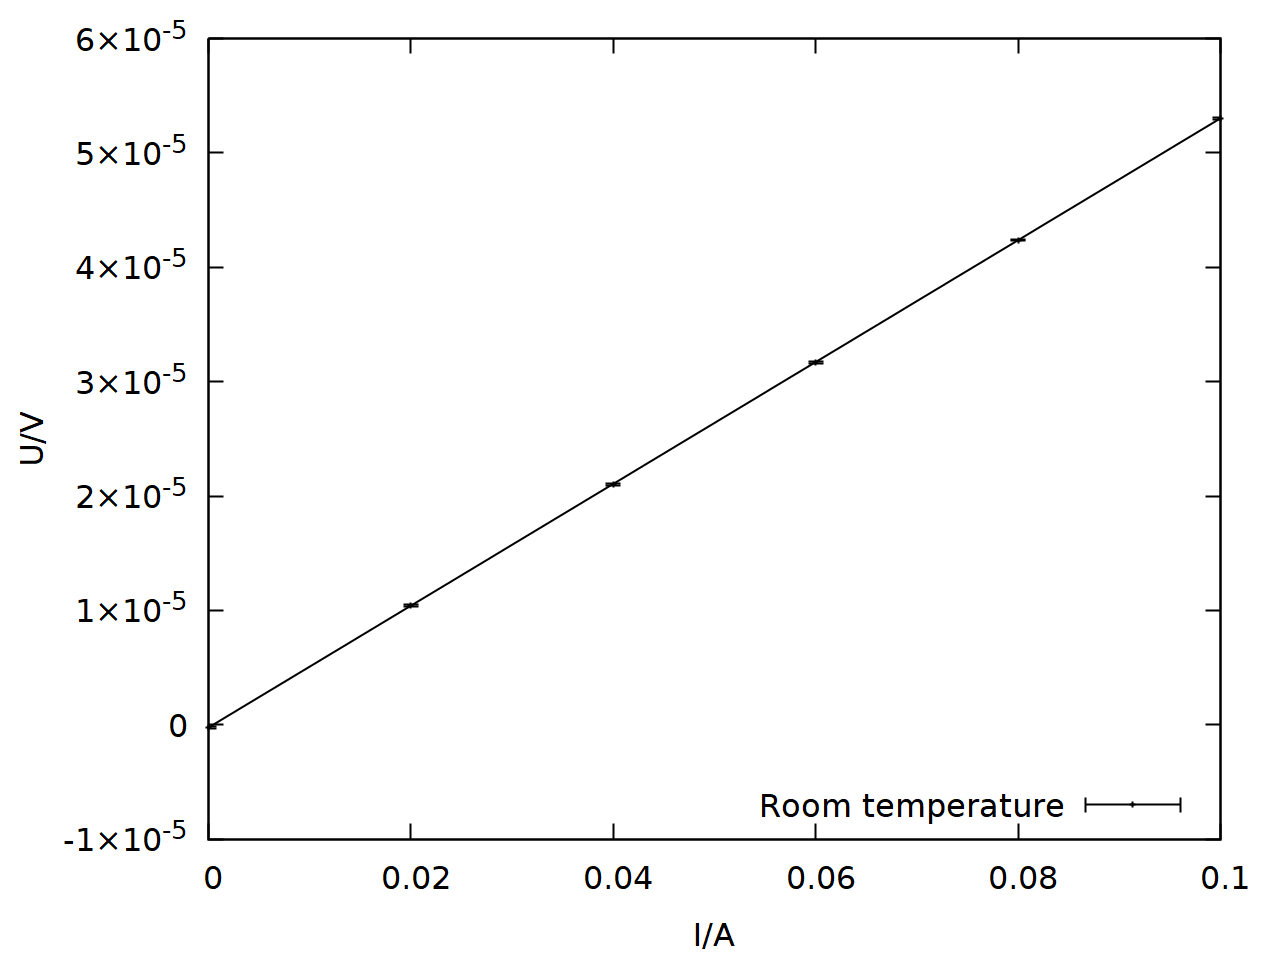
\includegraphics[width=0.7\linewidth]{data/elec.png}
    \caption{Resistivity: Voltage over current at room temperature}
    \label{fig:elec}
\end{figure}

In order to determine the resistivity we decided to plot the measured voltage over the current and to do a linear fit (see figure \ref{fig:elec}) rather than calculating the resistivity for each value and then taking the mean value. This has the advantage that we do not need to take any 'zero field' values into account explicitly.

The linear fit $f(x) = ax+b$ results in  $R = a = \si{(532.3\pm 0.4) \micro \Omega}$ and  $b = \si{(-2.5 \pm 0.2) \cdot 10^{-7} \Omega}$.

This leads to an resistivity of $\rho = \frac{R \cdot d \cdot b}{l\ind{R}} = \si{(1.85 \pm 0.08) \cdot 10^{-8} \Omega\meter}$.

\subsubsection{Thermal conductivity}

\begin{figure}
    \centering
    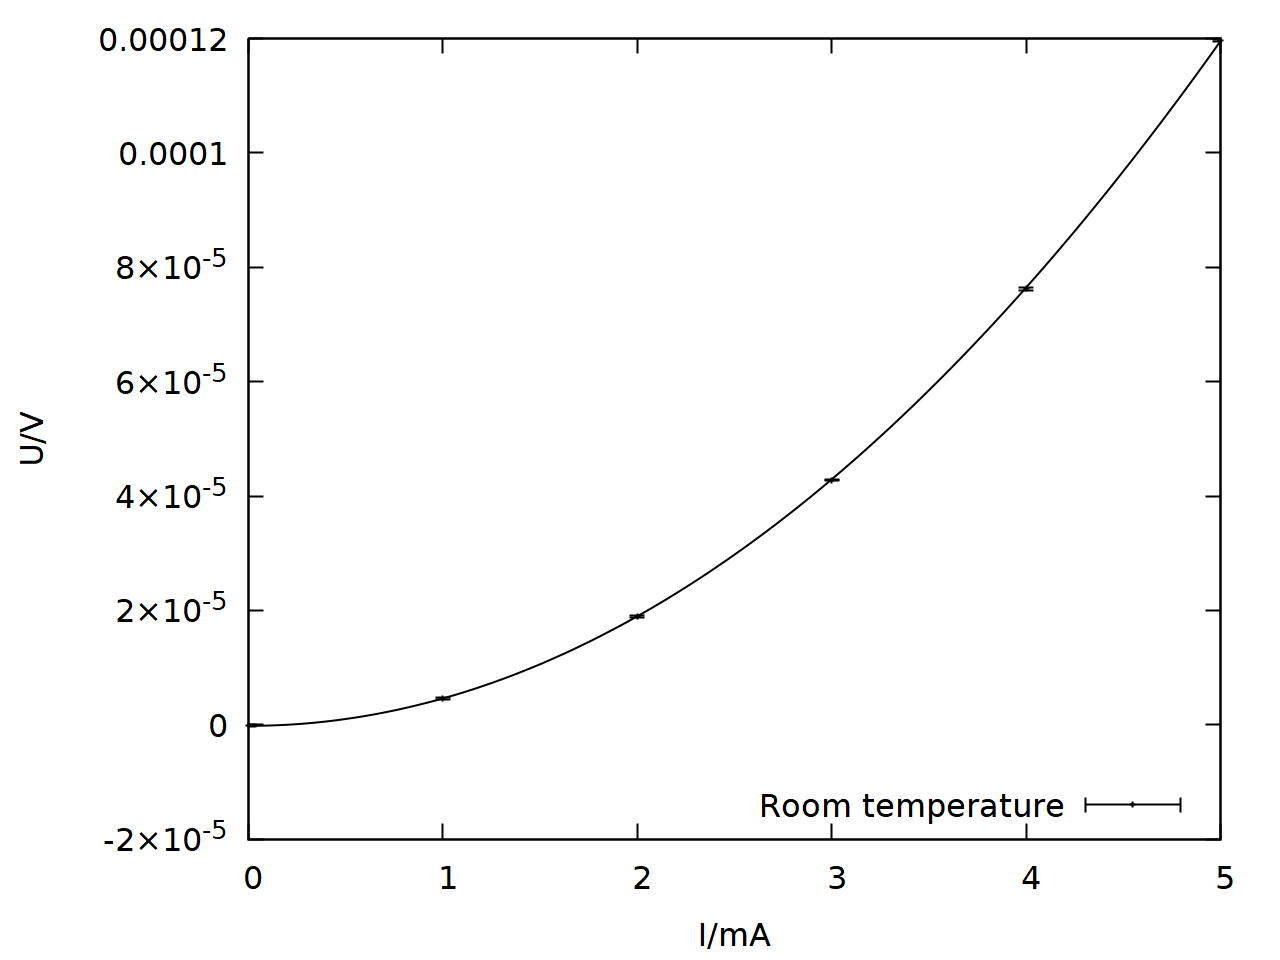
\includegraphics[width=0.7\linewidth]{data/therm.png}
    \caption{Thermal conductivity: Voltage over current at room temperature}
    \label{fig:therm}
\end{figure}

In figure \ref{fig:therm} the measured voltage is plotted over the current together with a quadratic fit $f(x) = ax^2 + b$. As expected the fit fits the data quite good. The parameters are $a = (4.789 \pm 0.005) V/A^2$ and $b = (-2.0 \pm 0.6) \cdot 10^{-8} \si{\volt}$. From this one can obtain $\kappa$ via $\kappa = \frac{S R\ind{PH} l\ind{TC}}{d\cdot b \cdot a} = (3614 \pm 64$)\,\si{W/Km}.

\subsection{Resistivity}
\begin{figure}
    \centering
    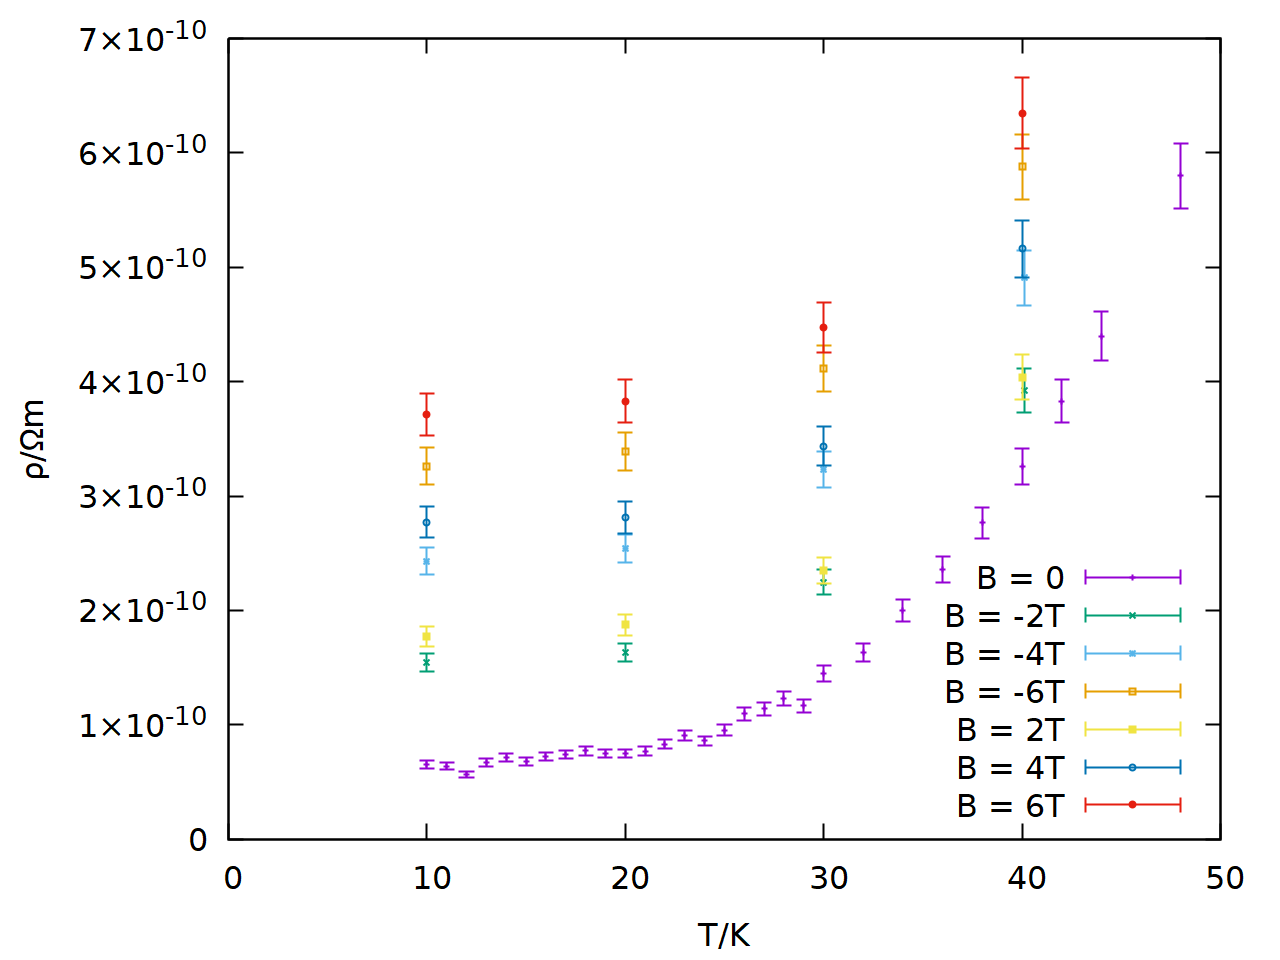
\includegraphics[width=0.7\linewidth]{data/rho_B.png}
    \caption{Resistivity over temperature for several magnetic fields}
    \label{fig:rho_B}
\end{figure}

In figure \ref{fig:rho_B} the resistivity is plotted for several magnetic fields. The resistivity increases with increasing magnetic field and temperature. There is a small difference between both directions of the magnetic field.

\begin{figure}
    \centering
    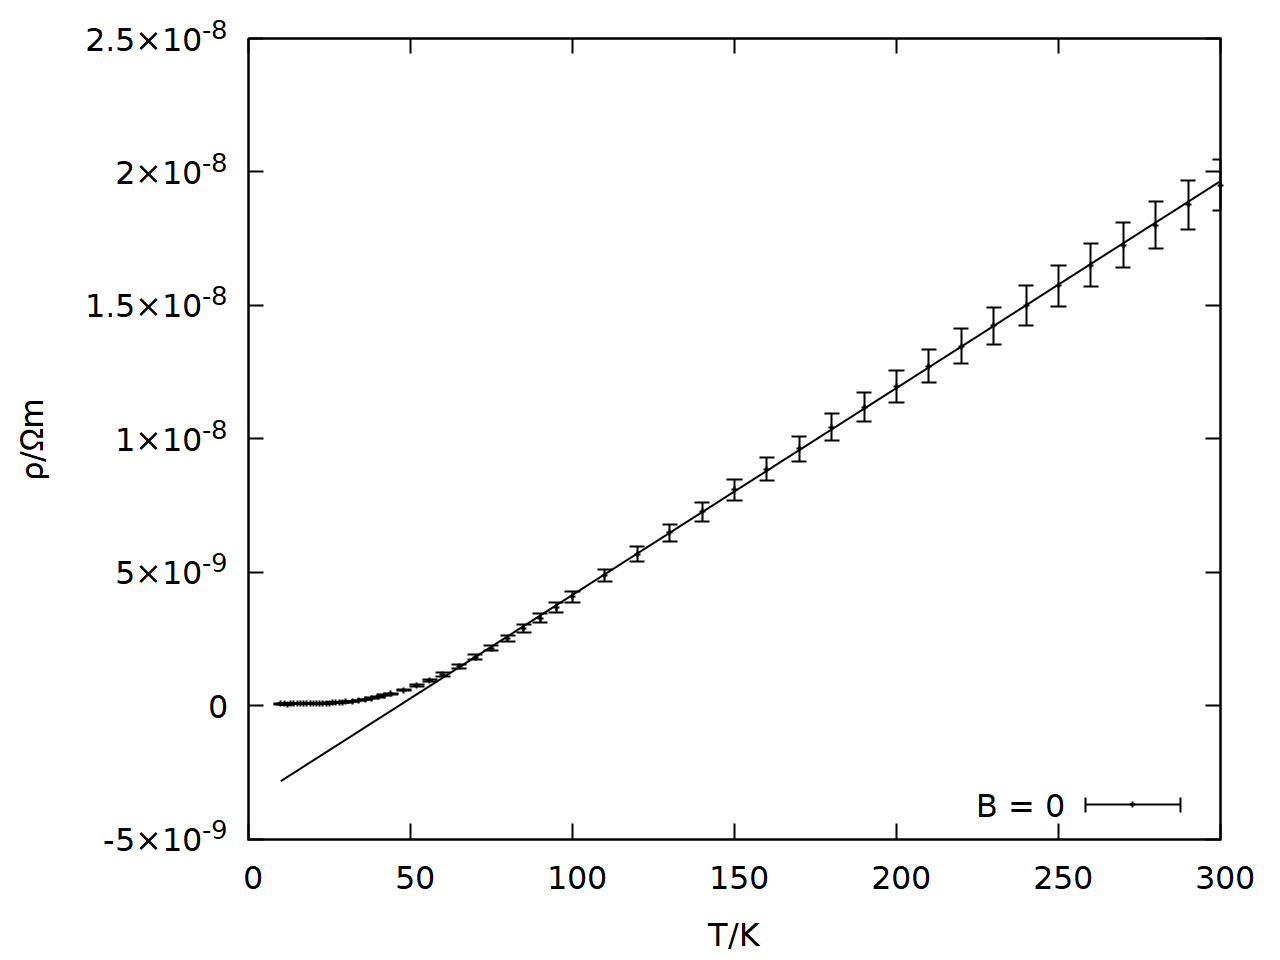
\includegraphics[width=0.7\linewidth]{data/rho_B0.png}
    \caption{Resistivity over temperature $B = 0$ with linear fit for $T > 100\si{\kelvin}$}
    \label{fig:rho_B0}
\end{figure}

In figure \ref{fig:rho_B0} the resistivity is plotted for $B = 0$ and higher temperatures. For $T \gtrapprox 100\,\si{\kelvin}$ the resisitivity is a linear function of temperature. A fit results in $\rho = (7.75 \pm 0.02)\cdot 10^-{-11} \si{\frac{\Omega m}{K}} \cdot T - (3.6 \pm 0.04) \cdot 10^{-9} \si{\Omega m}$

\begin{figure}
    \centering
    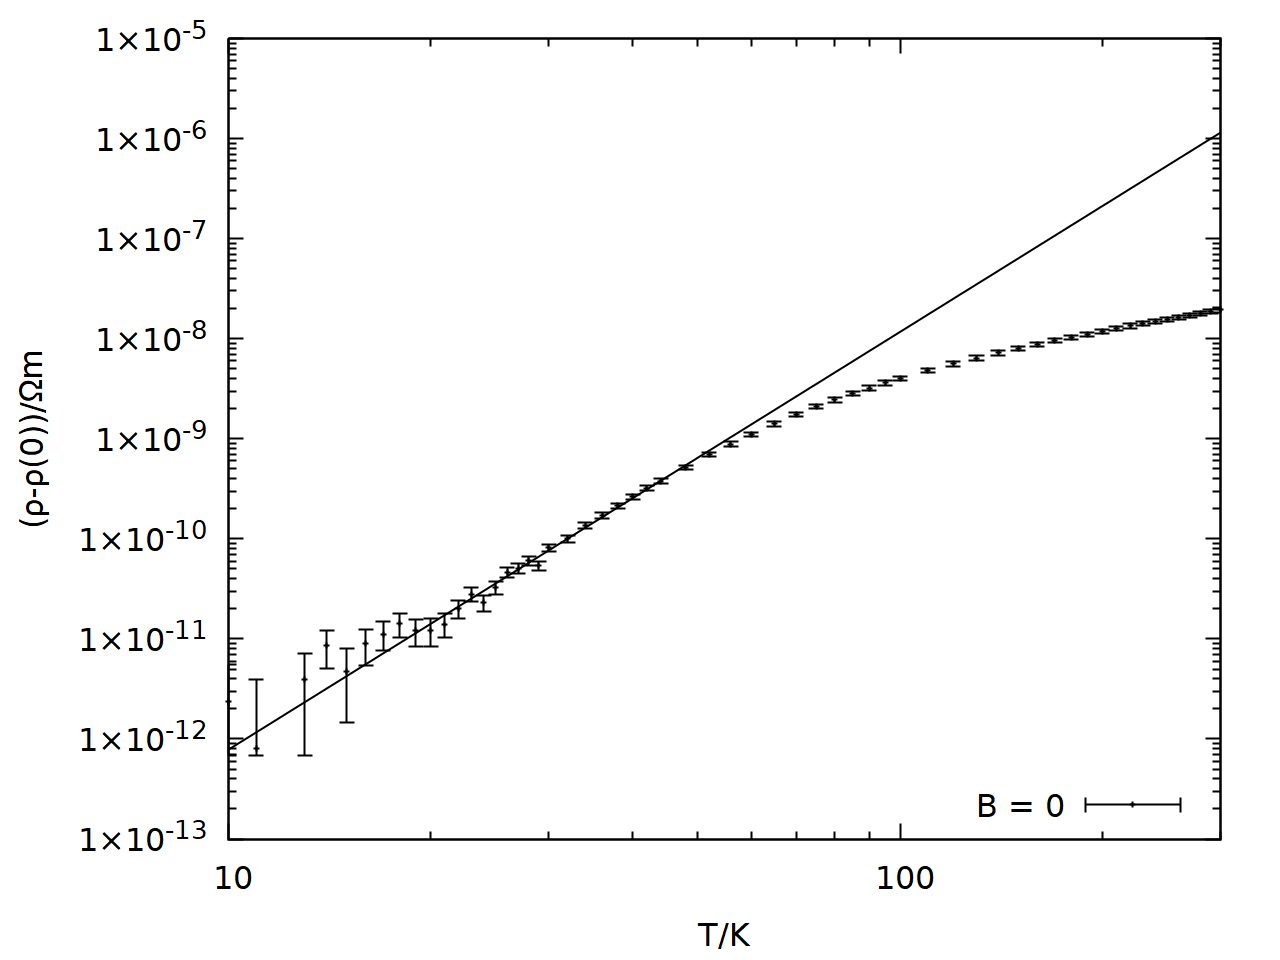
\includegraphics[width=0.7\linewidth]{data/rho_B0_fit.png}
    \caption{Resistivity over temperature $B = 0$ with polynomial fit for $T < 50\si{\kelvin}$}
    \label{fig:rho_B0_fit}
\end{figure}

For small temperatures ($T < 50 \si{\kelvin}$) we do a polynomial fit $f(x) = ax^b + c$ (This is basically the same as a linear fit in a double logarithmic diagram. However we do not need to guess the residual resistivity $c$ first and subtract it from the data.). As one can see in figure \ref{fig:rho_B0_fit} this fits the data well. The parameters are given by $a = (5 \pm 2) \cdot 10^{-17} \si{\frac{\Omega m}{K^b}}, b = (4.2 \pm 0.1), c = \rho(0) = (6.3 \pm 0.1) \cdot 10^{-11} \si{\Omega m}$.

Therefore the residual resistance is given by $\rho(0) = (6.3 \pm 0.1) \cdot 10^{-11} \si{\Omega m}$ which results in a $\mathrm{RRR} = \frac{\rho(300 \si{\kelvin})}{\rho(0)} = 310 \pm 17$. This is a quite high RRR value and therefore the sample has a good quality.

For low temperatures the resistivity behaves like $\rho \sim T^(4.2)$. In \cite{rho_low_temp} it is stated that the power is between $1 < b < 5$. Our result agrees with this.

\begin{figure}
    \centering
    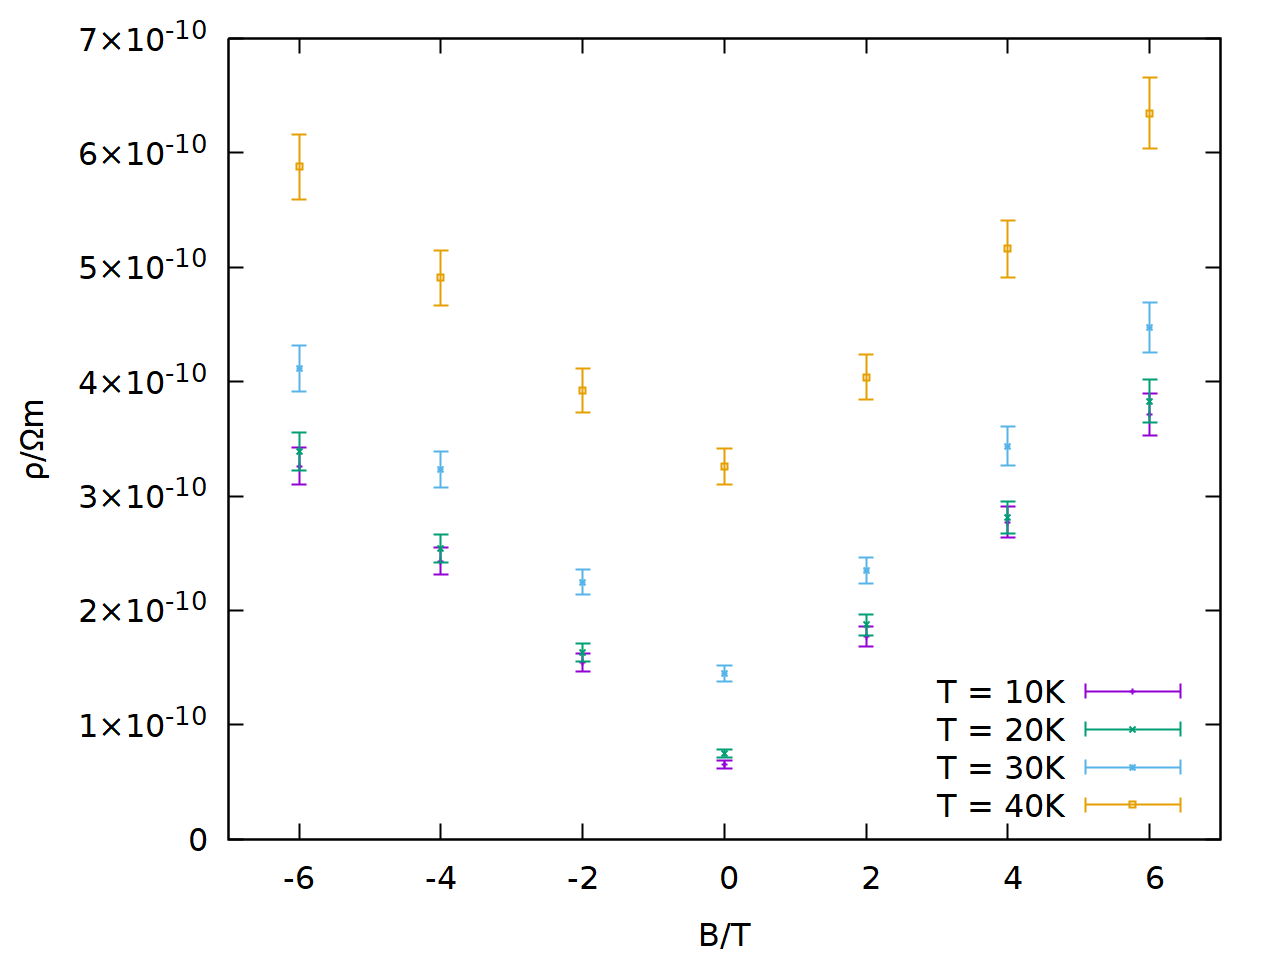
\includegraphics[width=0.7\linewidth]{data/rho_T.png}
    \caption{Resistivity over magnetic field for several temperatures}
    \label{fig:rho_T}
\end{figure}

In figure \ref{fig:rho_T} the resistivity is plotted over the magnetic field for several temperatures. As before the resisitivity increases with increasing magnetic field and temperature.

\subsection{Hall effect}

\begin{figure}
    \centering
    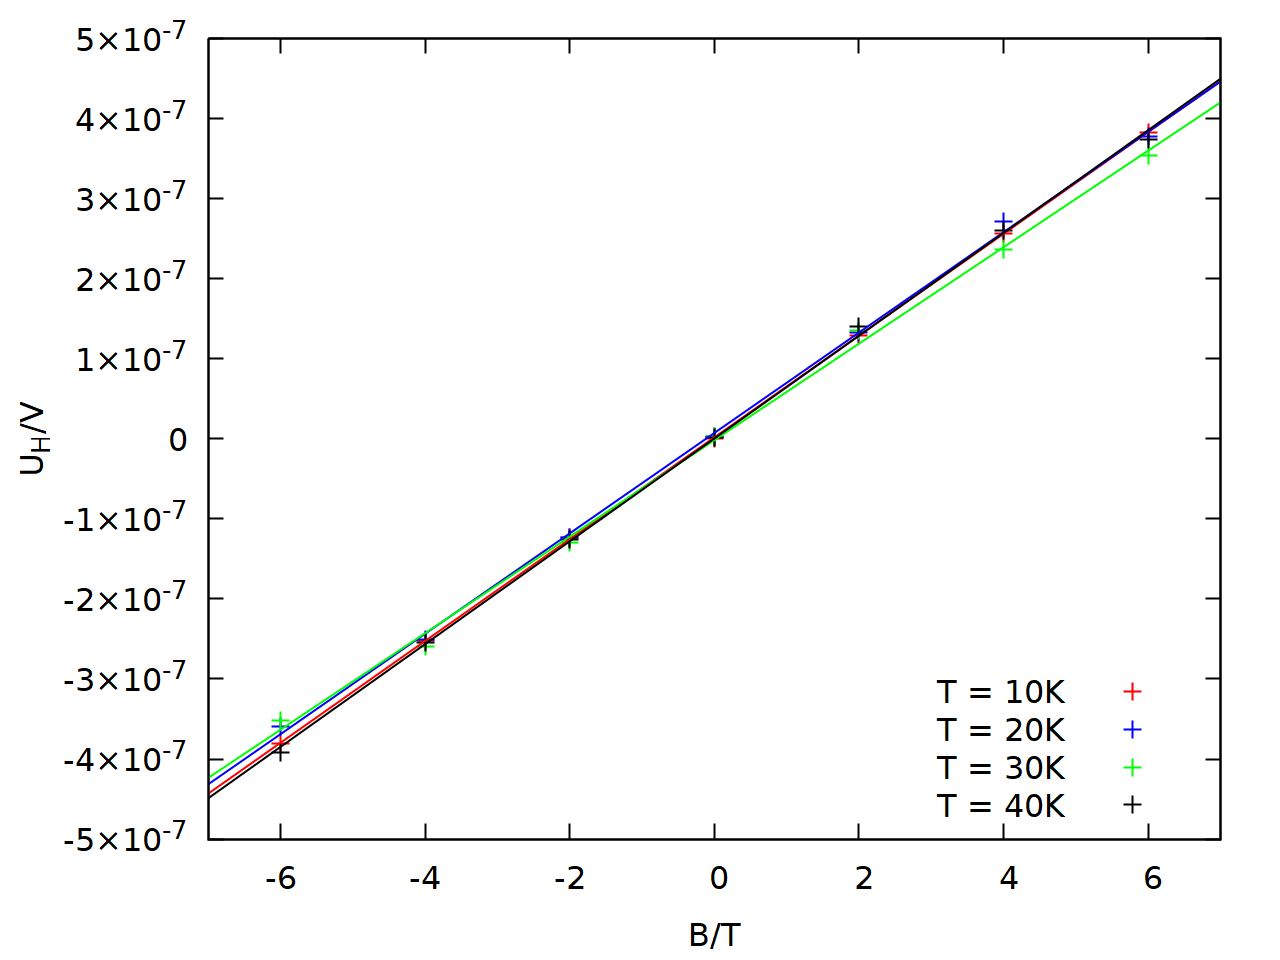
\includegraphics[width=0.7\linewidth]{data/rho_uh2_fit.png}
    \caption{Hall voltage over magnetic field for several temperatures with linear fits}
    \label{fig:rho_uh2_fit}
\end{figure}

In figure \ref{fig:rho_uh2_fit} the Hall voltage is plotted over the magnetic field for several temperatures. The Hall voltages do not significant change with temperature. The results of the linear fits $f(x) = ax + b$ are given in figure \ref{tab:rho_hall}.

\begin{table}[]
    \centering
    \begin{tabular}{ccccc}
    \toprule
    T/K & $a\cdot 10^8$/V/T & $b\cdot 10^9$/V & $A\ind{H}\cdot 10^{11}$ Vm/AT\\ 
    \midrule
    10 & 6.36 $\pm$ 0.01 & 1.9 $\pm$ 0.6 & 7.1 $\pm$ 0.1\\
    20 & 6.27 $\pm$ 0.08 & 7 $\pm$ 3 & 7.0 $\pm$ 0.1\\
    30 & 6.0 $\pm$ 0.1 & -2 $\pm$ 4 & 6.7 $\pm$ 0.1\\
    40 & 6.42 $\pm$ 0.08 & 0.5 $\pm$ 3 & 7.1 $\pm$ 0.1\\
    \bottomrule
    \end{tabular}
    \caption{Fit coefficients}
    \label{tab:rho_hall}
\end{table}

The Hall constant can be obtained from this by $A\ind{H} = a \cdot d/I$. The values for the Hall   constant vary only slightly with temperature. Their mean values is given by $\bar{A\ind{H}} = (7.0 \pm	0.2) \cdot 10^{-11} \si{Vm/TA}$.

\subsection{Thermal conductivity}
\begin{figure}
    \centering
    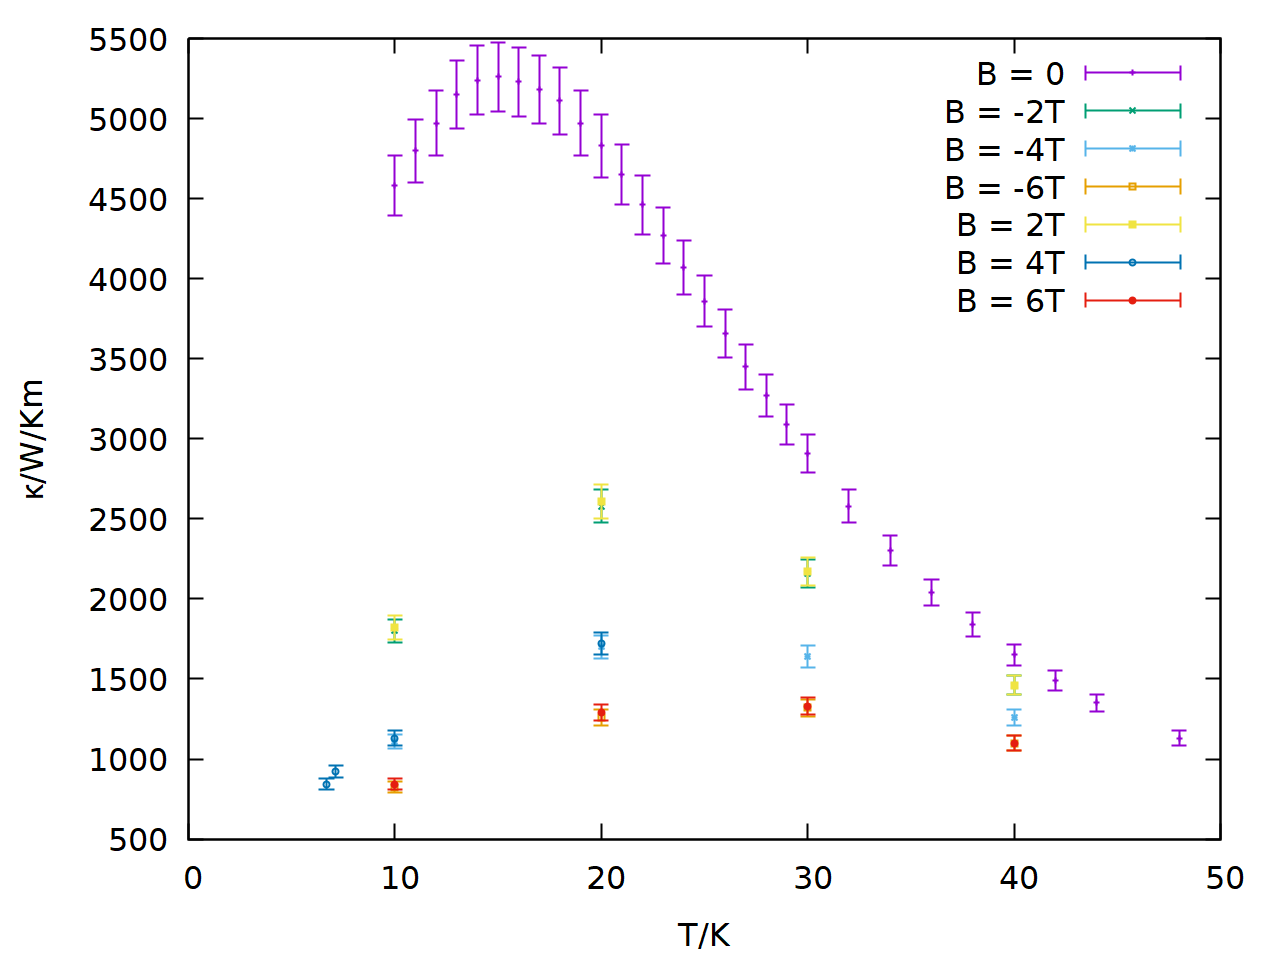
\includegraphics[width=0.7\linewidth]{data/wlf_B.png}
    \caption{Thermal conductivity over temperature for several magnetic fields}
    \label{fig:wlf_B}
\end{figure}

In figure \ref{fig:wlf_B} the thermal conductivity is plotted over the temperature for several magnetic fields. With increasing temperature it first grows but then drops. There is a small difference between both directions of the magnetic field, but they lie inside the errorbars.

\begin{figure}
    \centering
    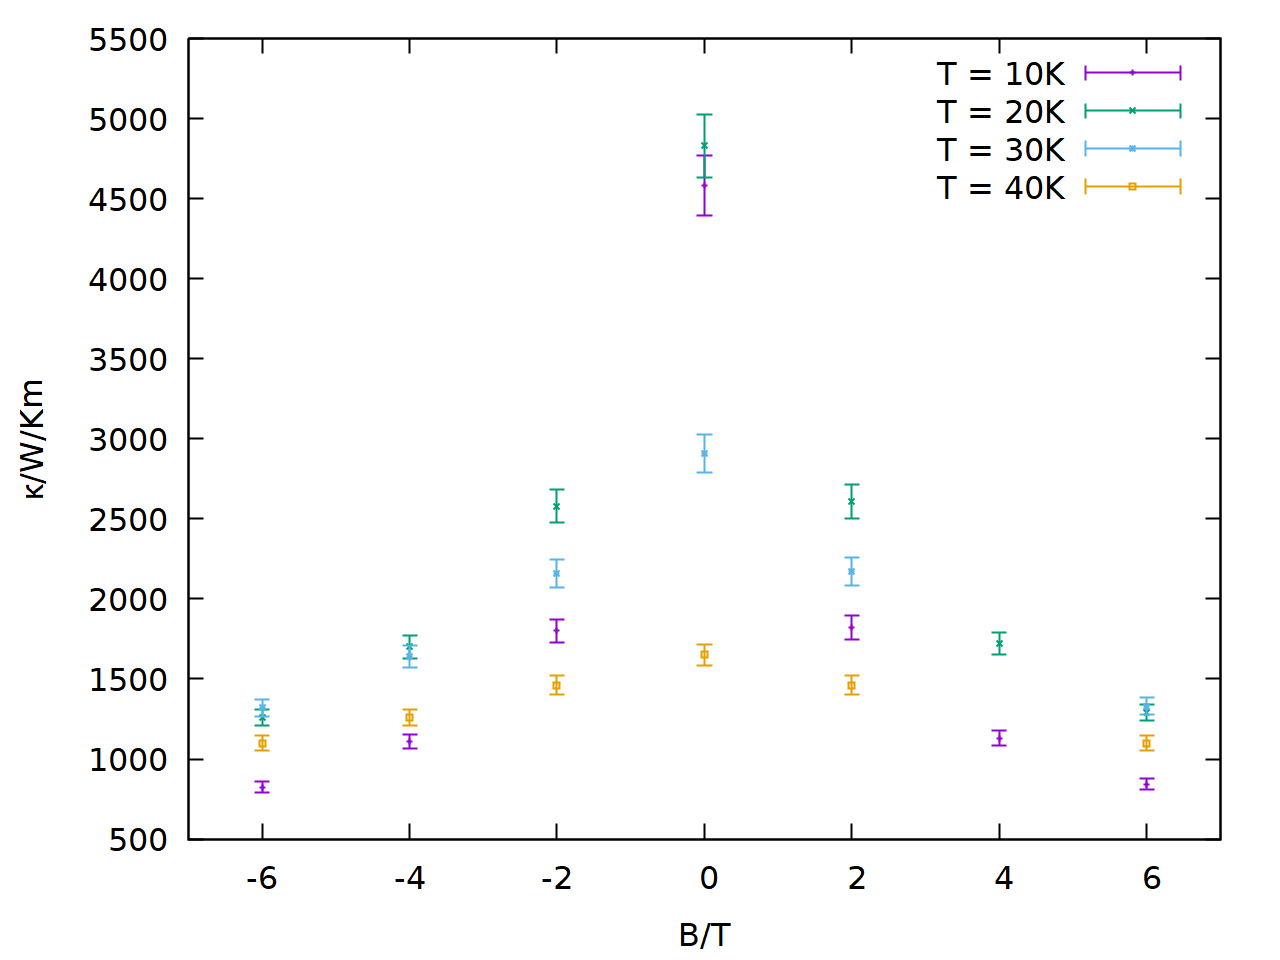
\includegraphics[width=0.7\linewidth]{data/wlf_T.png}
    \caption{Thermal conductivity over magnetic field for several temperatures}
    \label{fig:wlf_T}
\end{figure}

In figure \ref{fig:wlf_T} the thermal conductivity is plotted over the magnetic field for several temperatures. It drops with increasing magnetic field.

\subsection{Wiedemann-Franz law}

\begin{figure}
    \centering
    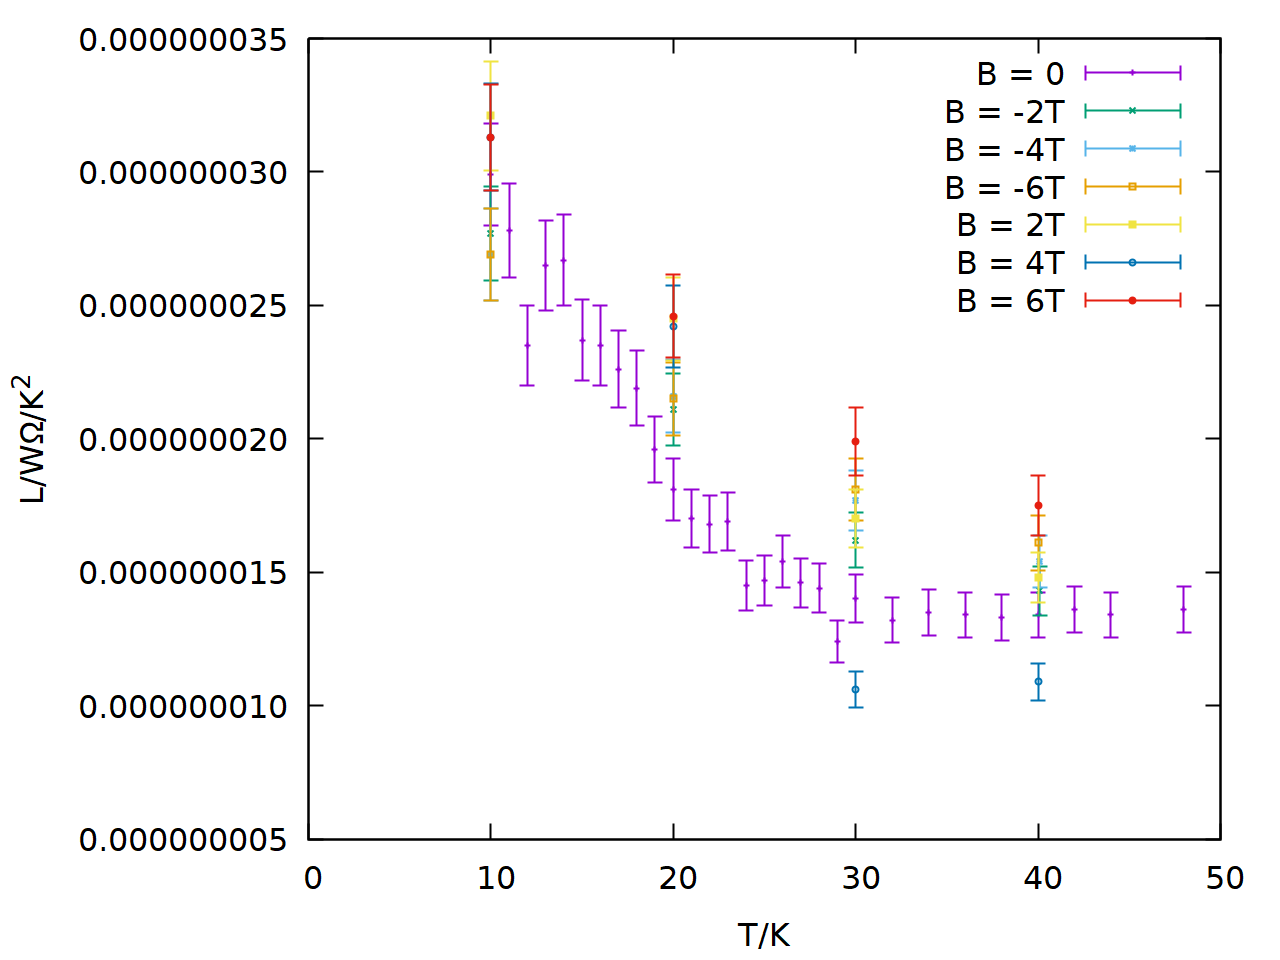
\includegraphics[width=0.7\linewidth]{data/wiede.png}
    \caption{Lorenz number L(T) for several magnetic fields}
    \label{fig:wiede}
\end{figure}

\begin{figure}
    \centering
    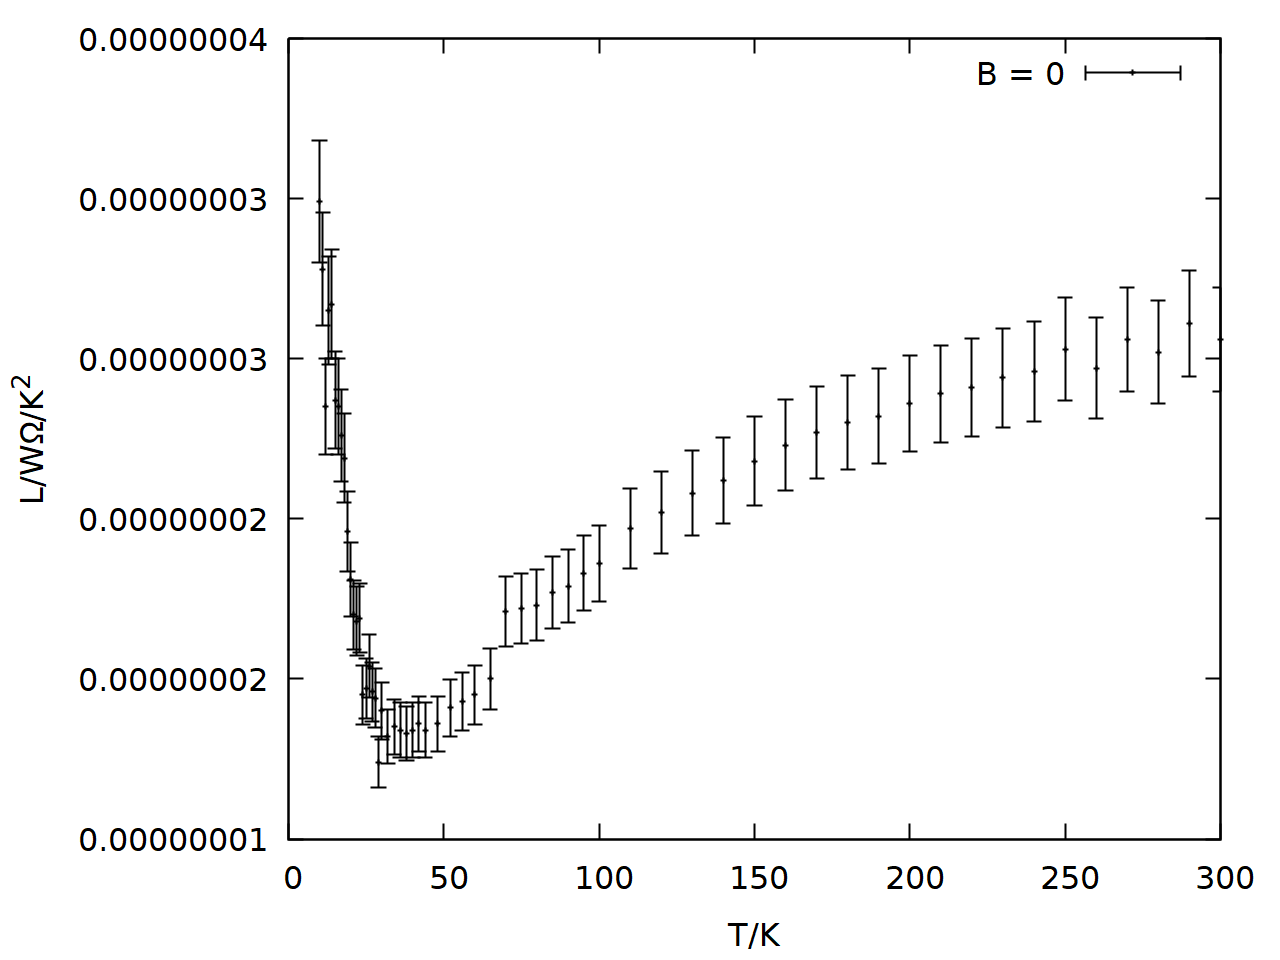
\includegraphics[width=0.7\linewidth]{data/wiede_B0.png}
    \caption{Lorenz number L(T) for $B = 0$}
    \label{fig:wiede_B0}
\end{figure}

\begin{figure}
    \centering
    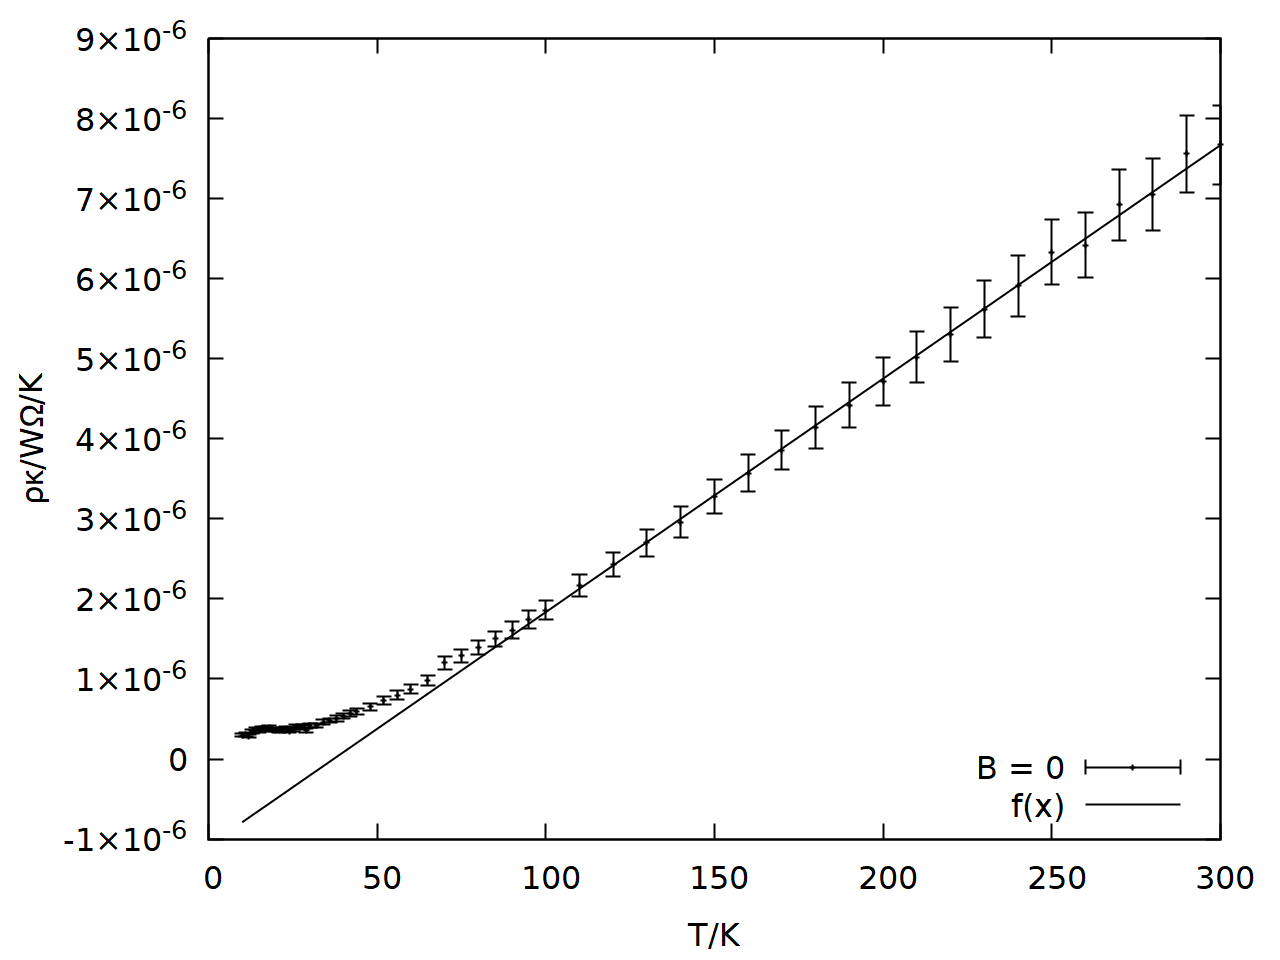
\includegraphics[width=0.7\linewidth]{data/wiede_B0_rhokappa.png}
    \caption{$\rho\kappa$ over $T$ for $B = 0$ with linear fit for $T > 100\si{K}$}
    \label{fig:wiede_B0_rhokappa}
\end{figure}

In figure \ref{fig:wiede} the Lorenz number $L = \frac{\kappa\rho}{T}$ is plotted for several magnetic fields. The values increase slightly with increasing field. Other than expected the Lorenz number is not a constant over temperature but rather drops. It gets even worse when plotting a greater temperature range (see figure \ref{fig:wiede_B0}). The values for $L$ are definitely not constant.

Therefore we decided not to plot $L$ but rather $\kappa\rho$ over $T$ (see figure \ref{fig:wiede_B0_rhokappa}). Now one can see a clearly linear dependence for higher temperatures. However the line does not cross $T= 0$ but is shifted by some value. A linear Fit $f(x) = ax+b$ for $T > 100 \si{K}$ results in $a = (2.92 \pm 0.02) \cdot 10^{-8} \si{W\Omega/K^2}, b = (-1.08 \pm 3) \cdot 10^6 \si{W\Omega/K}$. 

We will take $a = L = (2.92 \pm 0.02) \cdot 10^{-8} \si{W\Omega/K^2}$ as our measured value for the Lorenz factor. It differs a bit from the theoretical value $L = 2.44 \cdot 10^{-8} \si{W\Omega/K^2}$ \cite{wiede} but is in the same order of magnitude. Also note that the Wiedemann-Franz law is only an approximative law and the value of $L$ can vary from $2.1\cdot 10^{-8} \si{W\Omega/K^2} < L < 2.9\cdot 10^{-8} \si{W\Omega/K^2}$ \cite{wiede}. Therefore the deviation is not significant.

\subsection{Further analysis}
\subsubsection{Charge carrier density}
The charge carrier is given by $n = \frac{1}{\bar{A\ind{H} e}} = (9.0 \pm 0.3) \cdot 10^28 \si{m^{-3}}$. From this value on can obtain the Fermi velocity $v\ind{F} = \frac{\hbar}{m\ind{e}} (3\pi^2 n)^{1/3} = (1.4 \pm 0.4) \cdot 10^6 \frac{m}{s}$ and the Fermi energy $E\ind{F} = \frac{1}{2} m\ind{e} v\ind{F}^2 = (9.6\pm 0.3) \cdot 10^{-19} \si{J}$.

\subsubsection{Scattering time and mean free path}
The scattering time is given by $\tau = \frac{m\ind{e}}{e^2 n \rho}$, the mean free path by $\lambda = v\ind{F} \cdot \tau$. 

\begin{figure}
    \centering
    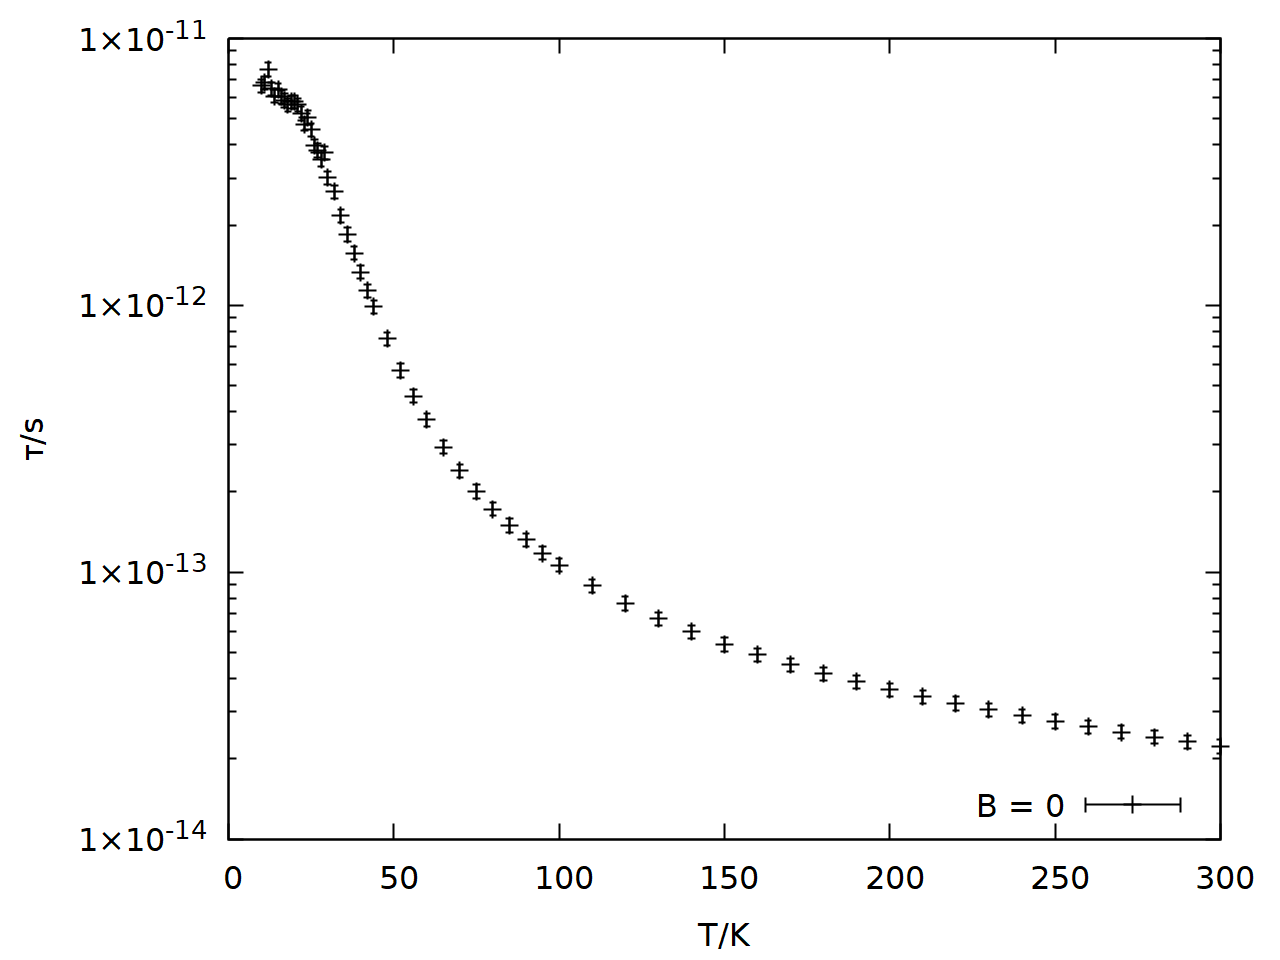
\includegraphics[width=0.7\linewidth]{data/rho_tau.png}
    \caption{Scattering time $\tau$ over $T$ for $B = 0$}
    \label{fig:rho_tau}
\end{figure}

\begin{figure}
    \centering
    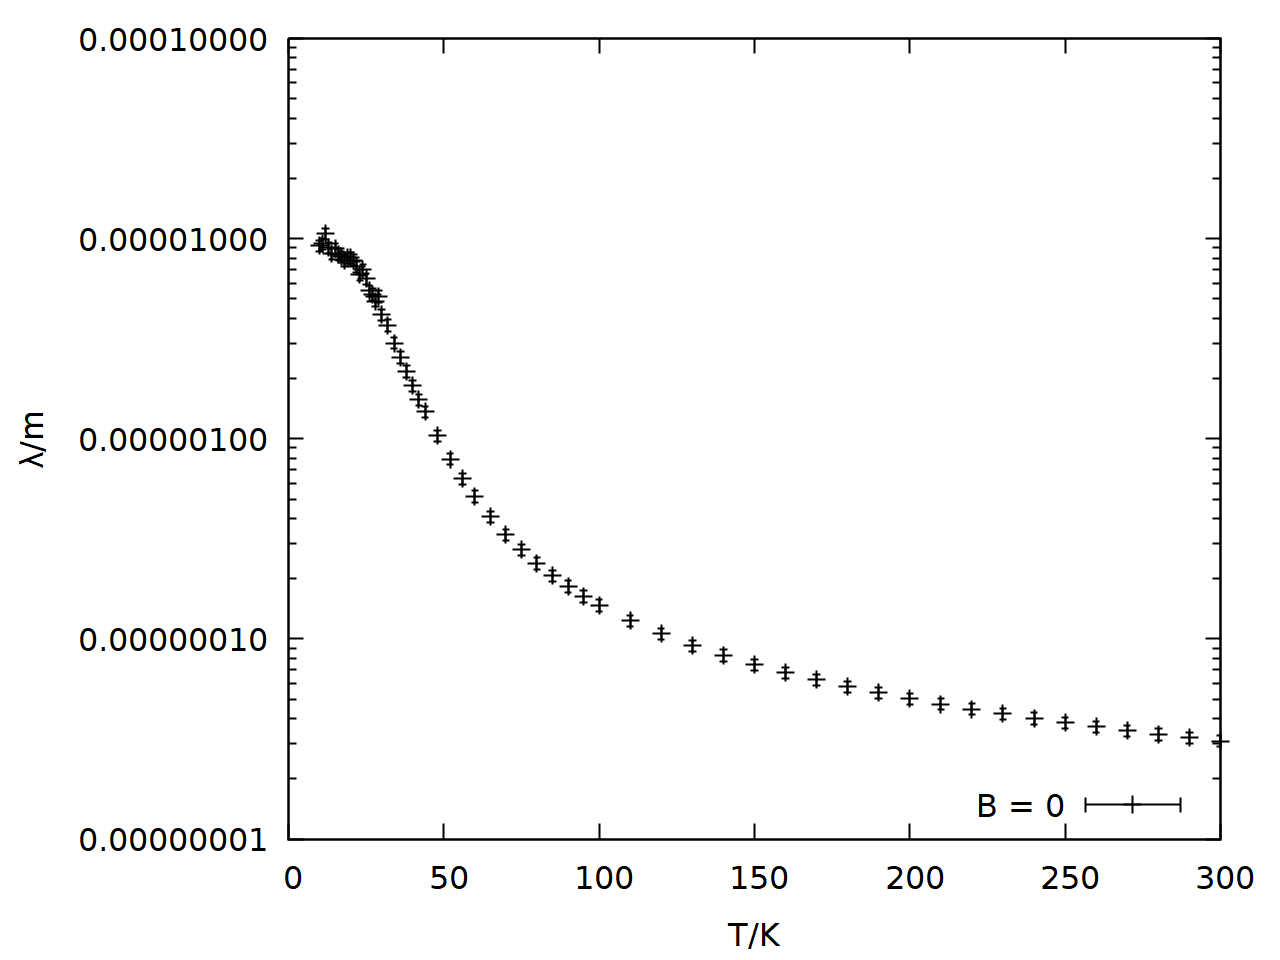
\includegraphics[width=0.7\linewidth]{data/rho_lambda.png}
    \caption{Mean free path $\lambda$ over $T$ for $B = 0$}
    \label{fig:rho_lambda}
\end{figure}

They are given in figures \ref{fig:rho_tau} and \ref{fig:rho_lambda} resp. One can easily see that they drop with increasing temperature as expected.
   